\newpage
\section{Fundatmental Of Flyback Converter}
\subsection{Basic Operating Principles}
\subsubsection*{Energy Storage in the Transformer During the ON Phase}
\begin{itemize}
    \item Explain that during the ON phase , when the switch (usually a MOSFET) is closed, current flows through the primary winding of the transformer.
    \item This current builds up a magnetic field in the transformer core, storing energy in the form of magnetic flux.
    \item The secondary winding is isolated during this phase, and no current flows to the output.
\end{itemize}
\begin{figure}[h!]
    \centering
    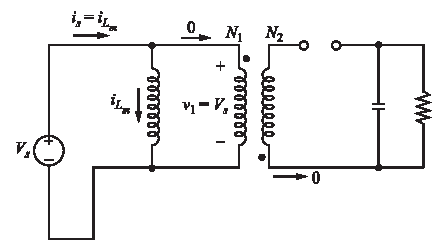
\includegraphics[width=0.6\linewidth]{Pictures/pics/4.pdf}
    \caption{\textcolor{blue}{\textit{\footnotesize  Circuit for the switch on.}}}
\end{figure}
\subsubsection*{Energy Transfer to the Output During the OFF Phase}
\begin{itemize}
    \item When the switch is turned OFF , the magnetic field collapses, inducing a voltage across the secondary winding.
    \item This voltage forward-biases the diode on the secondary side, allowing current to flow through the load and charge the output capacitor.
    \item The energy stored in the transformer is transferred to the output during this phase.
\end{itemize}
\begin{figure}[h!]
    \centering
    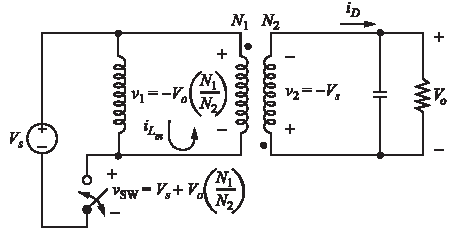
\includegraphics[width=0.6\linewidth]{Pictures/pics/5.pdf}
    \caption{\textcolor{blue}{\textit{\footnotesize   Circuit for the switch off.}}}
\end{figure}
\subsection{Key Components}
\begin{enumerate}
    \item \textbf{Transformer}: Stores energy during the ON phase and transfers it to the output during the OFF phase. Also provides voltage transformation and isolation.
    \item \textbf{Switch (MOSFET/IGBT)}: Controls the flow of current through the primary winding by turning ON and OFF.
    \item  \textbf{Diode (Output Rectifier)}: Rectifies the AC waveform from the secondary winding into DC.
    \item \textbf{Output Capacitor}:  Smooths the rectified output voltage and reduces ripple.
    \item \textbf{Input Capacitor}: smooths the input voltage and reduces ripple caused by pulsating current.
\end{enumerate}
\subsection{Modes of Operation}
\subsubsection*{Continuous Conduction Mode (CCM)}
\begin{itemize}
    \item In CCM, the current in the transformer never fully drops to zero during the OFF phase.
    \item This mode is typically used in higher-power applications because it reduces ripple current and improves efficiency.
    \item However, it requires more complex control and larger magnetics.
\end{itemize}
\subsubsection*{Discontinuous Conduction Mode (DCM)}
\begin{itemize}
    \item In DCM, the current in the transformer drops to zero before the next switching cycle begins.
    \item This mode is simpler to control and is often used in low-power applications.
    \item However, it can lead to higher peak currents and more EMI.
\end{itemize}
\subsubsection*{Boundary Conduction Mode (BCM)}
\begin{itemize}
    \item BCM operates at the boundary between CCM and DCM, where the current just reaches zero at the end of the OFF phase.
    \item This mode offers a balance between efficiency and simplicity, making it popular in medium-power applications.
\end{itemize}
